% Indicate the main file. Must go at the beginning of the file.
% !TEX root = ../main.tex

%%%%%%%%%%%%%%%%%%%%%%%%%%%%%%%%%%%%%%%%%%%%%%%%%%%%%%%%%%%%%%%%%%%%%%%%%%%%%%%%
% 04_discussion
%%%%%%%%%%%%%%%%%%%%%%%%%%%%%%%%%%%%%%%%%%%%%%%%%%%%%%%%%%%%%%%%%%%%%%%%%%%%%%%%


\section{Discussion}
\label{discussion}

\subsection{Hyperparameter Tuning}%%%%%%%%%%%%%%%%%%%%%%%%%%%%%%%%%%%%%%%%%%%%%%

The detailed results of the Hyperparameter tuning are shown in \autoref{tab:hyperparameters_results}.
It is quite difficult to find any obvious tendencies for the influence of the
hyperparameters on the performance of the model. There is no direct correlation
between the model size and the performance of the model. This might be explicable
by the fact that the available data is not sufficient to train larger models.
This could be helped by extending the dataset with additional recordings or by
implementing some sort of data augmentation. Some ideas being to add random levels
of noise to the recordings or to randomly add slight shifts in time or frequency.
An other approach could be to mix data from different classes to create new samples.
This would have two main advantages. First the combination possibilities are endless
and therefore the dataset could be extended massively. Second the model would be
trained to to detect multiple classes in one sample wich could be useful in a real
world scenario where multiple species are present at the same time. In order to
implement this, the output layer of the model must be changed - specifically the
softmax activation function must be replaced by a sigmoid activation function.
The data augmentation could be implemented in the dataloader to be done on the fly.

An other thing to look into is the selection of the hyperparameters. Dew to limited
resources the hyperparameter tuning was done with a limited number of configurations.
There is still a list of potential hyperparameters that could be tested. As an example
the base channels after the in layer or different parameters for the transformation
such as the hop length, window size or the number of mel bins. As the model is, the
kernel size stays the same for all layers - the possibilities there are endless.

\subsection{Performance of the best Model}%%%%%%%%%%%%%%%%%%%%%%%%%%%%%%%%%%%%%%

Using the best performing configuration it is worth to take a closer look to the
training process of the model. The validation accuracy and loss at the end of
every epoch is shown in \autoref{fig:loss_acc_best}. The graphs show a typical
training process. The validation accuracy is increasing while the validation loss
is decreasing. Towards the end both graphs are flattening out which is a sign that
the model was not learning anymore when the training was stopped. So the patience
of 100 for the early stopping was an appropriate choice. Since the validation loss
and accuracy are very noisy it was necessary to use a patience that high. This might
be a sign, that the data processing or the model architecture could be improved.

%==== figure: loss_acc_best ====%
\begin{figure}[h]
\centering
\captionsetup{width=0.9\linewidth}
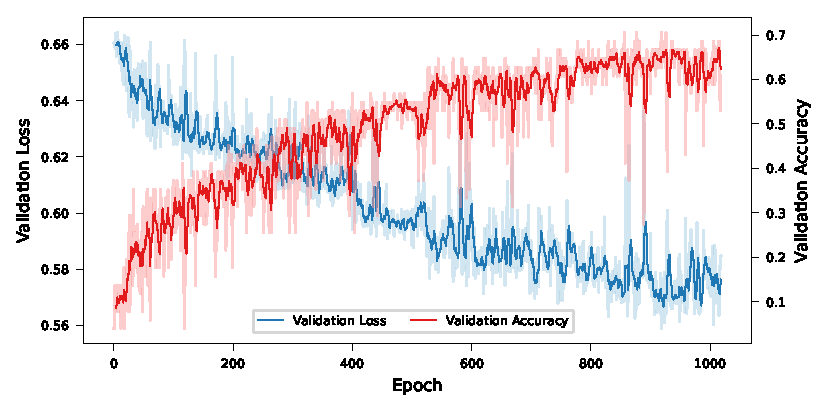
\includegraphics[width=1.0\textwidth]{figures/loss_acc_best.pdf}
\caption{The validation loss and accuracy of the best model. Light version is not smoothed and dark version is smoothed with a window size of 5.}
\label{tab:loss_acc_best}
\end{figure}

%===============================%

In the original paper \autocite{faissAdaptiveRepresentationsSound2023}
the model was used on different datasets and with different models. Furthermore the model was
run five times with different seeds and the accuracy was averaged. The model using a MelSpectrogram
frontend on the InsectSet32 dataset achieved an mean accuracy of 0.6 with a range of 0.57 to 0.65
on the validation set and an accuracy of 0.62 with a range of 0.57 to 0.67 on the test set.
The best performing configuration for the model in this study achieves an accuracy of 0.706 on the validation set
and an accuracy of 0.649. For the test set this is well in the range of the original paper.
Why the model in this study performs better on the validation set compared to the difference
between the validation and test set in the original paper is not clear. The accuracy achieved
by the model with the other frontend from the original paper is unreached by the model in this study.
So there is still room for improvement especially in the data processing.

\subsection{Sum Up}%%%%%%%%%%%%%%%%%%%%%%%%%%%%%%%%%%%%%%%%%%%%%%%%%%%%%%%%%%%%

To sum up, the model was successfully trained and evaluated. The results are comparable to the results
of the original paper. The model is able to classify the sounds of a limited subset of insects with an accuracy of 0.649.
This was all done on a regular gaming computer with a GPU by a student with none to little experience
in the field of deep learning - notbabel with quite some demand for support.
Still it is save to say that this technology has become accessible to everyone 
with the knowledge and some quite affordable hardware.
